\documentclass[tikz,border=5mm]{standalone}
\usetikzlibrary{decorations.markings}

\begin{document}
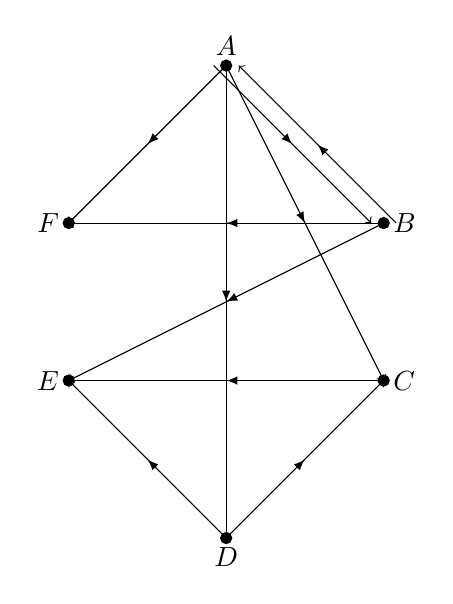
\begin{tikzpicture}
    \tikzset{
        myarrow/.style={
            postaction={
                decorate,
                decoration={
                    markings,
                    mark=at position #1 with {\arrow{latex}},
                },
            },
        },
    }

    % Vertices
    \draw[fill=black] (4, 6) circle (2pt) node[above] {$A$};
    \draw[fill=black] (6, 4) circle (2pt) node[right] {$B$};
    \draw[fill=black] (6, 2) circle (2pt) node[right] {$C$};
    \draw[fill=black] (4, 0) circle (2pt) node[below] {$D$};
    \draw[fill=black] (2, 2) circle (2pt) node[left] {$E$};
    \draw[fill=black] (2, 4) circle (2pt) node[left] {$F$};

    % Arcs
    \draw[->, myarrow=.5, transform canvas={xshift=-4.5pt}] (4,6) -- (6,4);
    \draw[->, myarrow=.5, transform canvas={xshift=+4.5pt}] (6,4) -- (4,6);
    \draw[->, myarrow=.5] (4,6) -- (6,2);
    \draw[->, myarrow=.5] (4,6) -- (4,0);
    \draw[->, myarrow=.5] (4,6) -- (2,4);
    \draw[->, myarrow=.5] (6,4) -- (2,2);
    \draw[->, myarrow=.5] (6,4) -- (2,4);
    \draw[->, myarrow=.5] (6,2) -- (2,2);
    \draw[->, myarrow=.5] (4,0) -- (2,2);
    \draw[->, myarrow=.5] (4,0) -- (6,2);

\end{tikzpicture}
\end{document}
